% vim: expandtab softtabstop=2 shiftwidth=2 foldmethod=marker spell


\documentclass{article}
\usepackage{fancyhdr}
\usepackage{multirow}   %helps with tables, allows for multiple rows to combine
\usepackage{amssymb}    %allows for the use of \square which makes a blank square in long multiplication
\usepackage[hidelinks, letterpaper, pagebackref, bookmarksopen, bookmarksnumbered]{hyperref} %makes table of contents
\usepackage{bookmark}                                                                        %helps with table of contents
\usepackage{import}
\usepackage{booktabs}
\usepackage{pgfplotstable}
\usepackage{booktabs, colortbl}
\usepackage{tikz}
\usepackage{cellspace}
\setlength\cellspacetoplimit{3pt}
\setlength\cellspacebottomlimit{3pt}
\usepackage{amsmath}
\usepackage{listings}
\usepackage{color}

\definecolor{codegreen}{rgb}{0,0.6,0}
\definecolor{codegray}{rgb}{0.5,0.5,0.5}
\definecolor{codepurple}{rgb}{0.58,0,0.82}
\definecolor{backcolour}{rgb}{0.95,0.95,0.92}
 
\lstdefinestyle{mystyle}{
    backgroundcolor=\color{backcolour},   
    commentstyle=\color{codegreen},
    keywordstyle=\color{magenta},
    numberstyle=\tiny\color{codegray},
    stringstyle=\color{codepurple},
    basicstyle=\footnotesize,
    breakatwhitespace=false,         
    breaklines=true,                 
    captionpos=b,                    
    keepspaces=true,                 
    numbers=left,                    
    numbersep=5pt,                  
    showspaces=false,                
    showstringspaces=false,
    showtabs=false,                  
    tabsize=2
}
 
\lstset{style=mystyle}

\def\mydate{\leavevmode\hbox{\the\year-\twodigits\month-\twodigits\day}}
\def\twodigits#1{\ifnum#1<10 0\fi\the#1}
\title{Guide to the Songbot}
\date{\mydate}

\fancypagestyle{plain}
{
  \fancyhf{}
  \lfoot{\author{Guide to the Songbot}}
  \cfoot{\thepage}
  \rfoot{\date{\mydate}}
  \renewcommand{\headrulewidth}{0pt}
}
\pagestyle{plain}

\begin{document}
\maketitle
\newpage
\pdfbookmark[section]{\contentsname}{toc}
\tableofcontents
\clearpage

% vim: expandtab softtabstop=2 shiftwidth=2 foldmethod=marker spell

\section{Turning the songbot on and off}
For small communities where the chat moves slowly, the best practice for turning the songbot on and off is to use the chat command \lstinline{!setrequests on/off}. This lets the streamer see that the bot is turned on or off. There is also a shortcut for the command \lstinline{!srs on/off}. It is important to note that mods can add songs when requests are off.

\begin{figure}[ht!]
  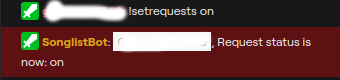
\includegraphics[width=\linewidth]{src/songbot_on_off/setrequests_on.png}
  \caption{The chat messages to turn on the songbot}
  \label{setrequests on}
\end{figure}
\begin{figure}[ht!]
  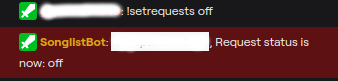
\includegraphics[width=\linewidth]{src/songbot_on_off/setrequests_off.png}
  \caption{The chat messages to turn off the songbot}
  \label{setrequests off}
\end{figure}
\begin{figure}[ht!]
  
\includegraphics[width=\linewidth]{src/songbot_on_off/request_failed.png}
  \caption{The chat messages when a request fails because the songbot is off}
  \label{request failed}
\end{figure}

\newpage

An alternative to the chat commands is to use the web interface of \mbox{streamersonglist}.
\begin{figure}[ht!]
  \includegraphics[width=\linewidth]{src/songbot_on_off/bot_on.png}
  \caption{The webpage with the songbot turned on}
  \label{bot is on}
\end{figure}
\begin{figure}[ht!]
  \includegraphics[width=\linewidth]{src/songbot_on_off/bot_off.png}
  \caption{The webpage with the songbot turned off}
  \label{bot is off}
\end{figure}


\clearpage
% vim: expandtab softtabstop=2 shiftwidth=2 foldmethod=marker spell

\section{Importing Songs}
How to import songs from a CSV (Comma Separated Values) file.

A CSV file is literally its name, just a bunch of things separated by commas. Due to its very simple nature, CSV files can be edited with most programs including Wordpad, but common editors include Google Sheets and Microsoft Excell.

In the table below, you can see what an example of a comma separated values songlist would look like. 
The first line of the file names the columns, such as title, artist, and active. 

\begin{table}[h!]
\pgfplotstabletypeset[col sep=comma,
  string type,
  columns={title,artist,active},
  every head row/.style={before row=\hline,after row=\hline},
  every last row/.style={after row=\hline},
  every even row/.style={before row=\rowcolor[gray]{0.9}},
  every first column/.style={column type/.add={|}{}},
  every column/.style={column type/.add={}{|}},
  ]{src/songlist_import/example.csv}
\caption{Songlist Example CSV}
\label{example.csv}
\end{table}

Active is a bit special in that it uses a classical boolean value. 
A 0 represents that the song is off or inactive, and a 1 represents that song is on or active.
An inactive song can is no longer shown as part of the normal songlist, but instead can be seen by mods and above in edit mode. 
They will be displayed in red when the "show inactive" slider is active.

\begin{figure}[ht!]
  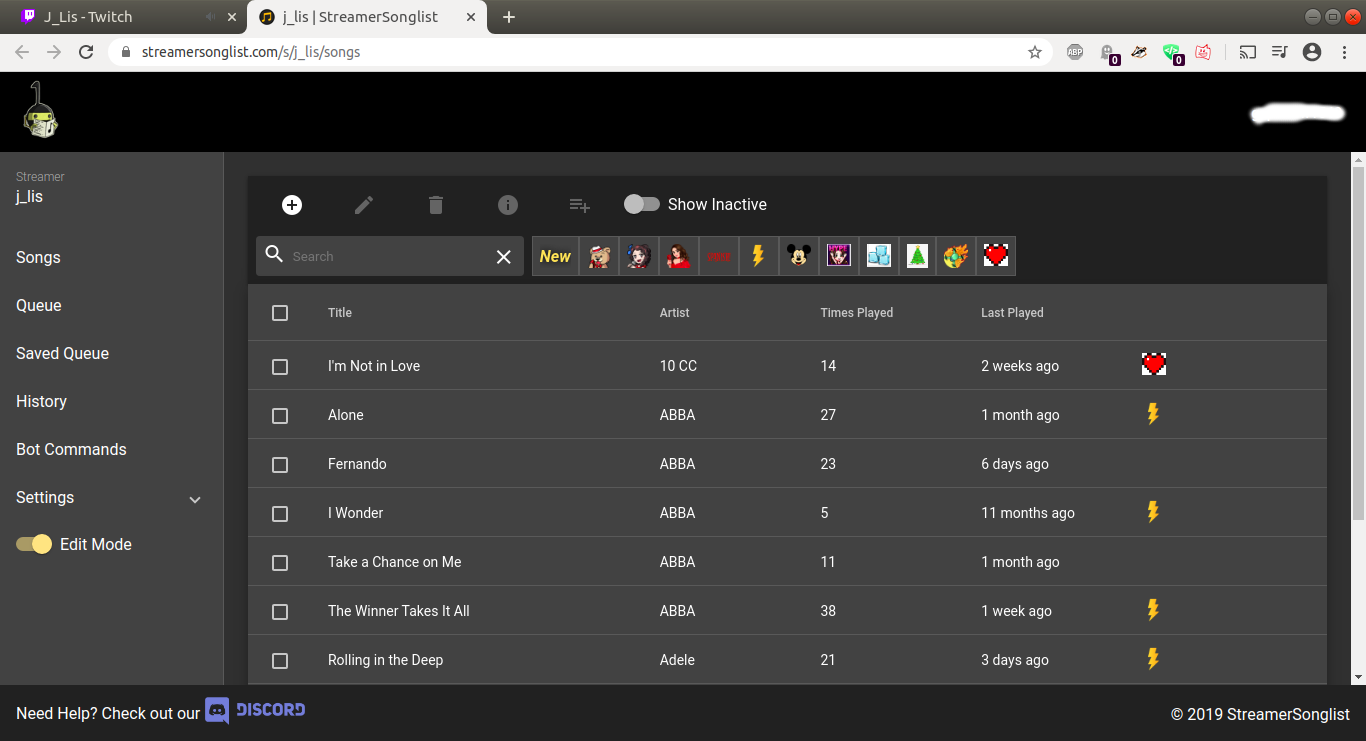
\includegraphics[width=\linewidth]{src/songlist_import/songlist_main_edit.png}
  \caption{The "show inactive" slider}
  \label{show inactive}
\end{figure}

Once your songlist is created as a CSV, you can add it from the import songs page.

\begin{figure}[ht!]
  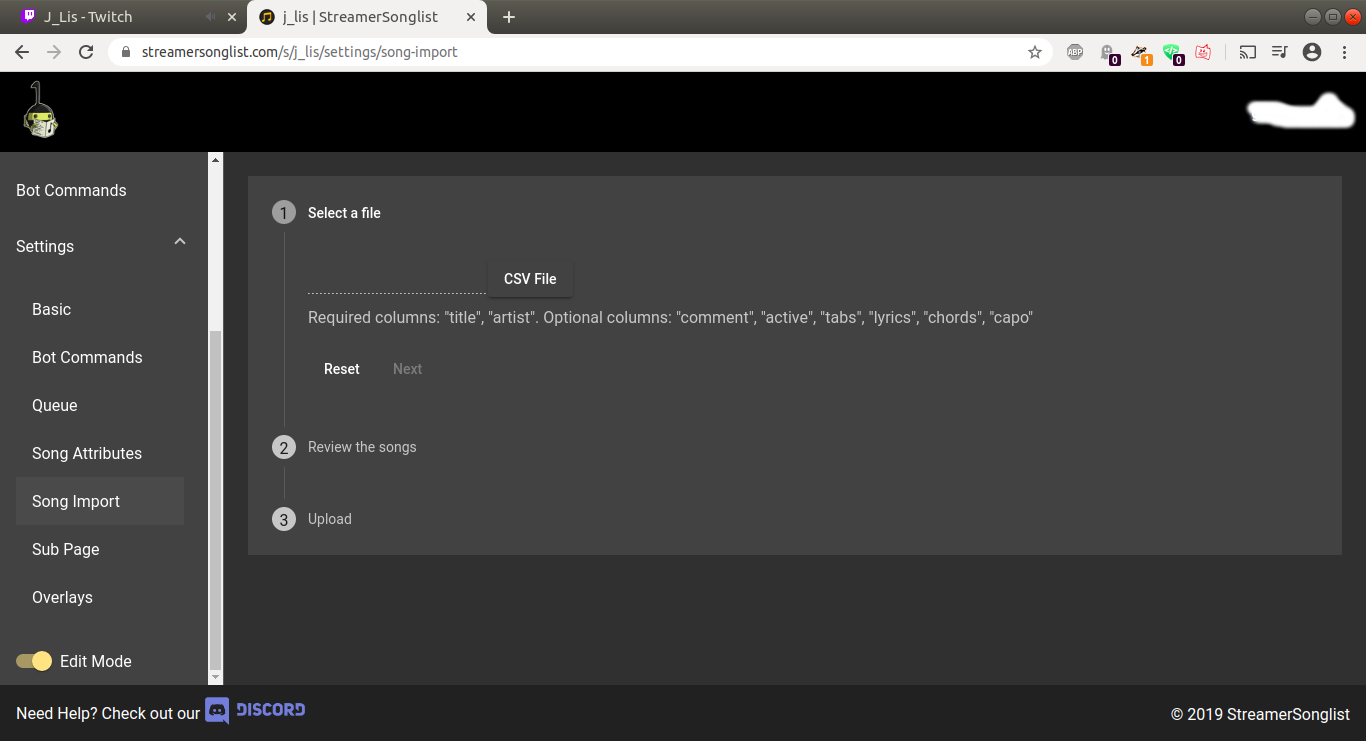
\includegraphics[width=\linewidth]{src/songlist_import/import_songs.png}
  \caption{The import songs page}
  \label{import songs}
\end{figure}

\clearpage
% vim: expandtab softtabstop=2 shiftwidth=2 foldmethod=marker spell

\section{Troubleshooting the songbot}

\subsection{Normal users cant add songs}

Step one, use the command \lstinline{!sl}, which should return the link to the songlist. If it does, check to see if the queue is on.
\begin{figure}[ht!]
  \includegraphics[width=\linewidth]{src/troubleshooting_songbot/bot_off.png}
  \caption{The webpage with the songbot turned off}
  \label{bot is off}
\end{figure}

When the command \lstinline{!sl} does not work, check to see if the bot is connected to chat.
\begin{figure}[ht!]
  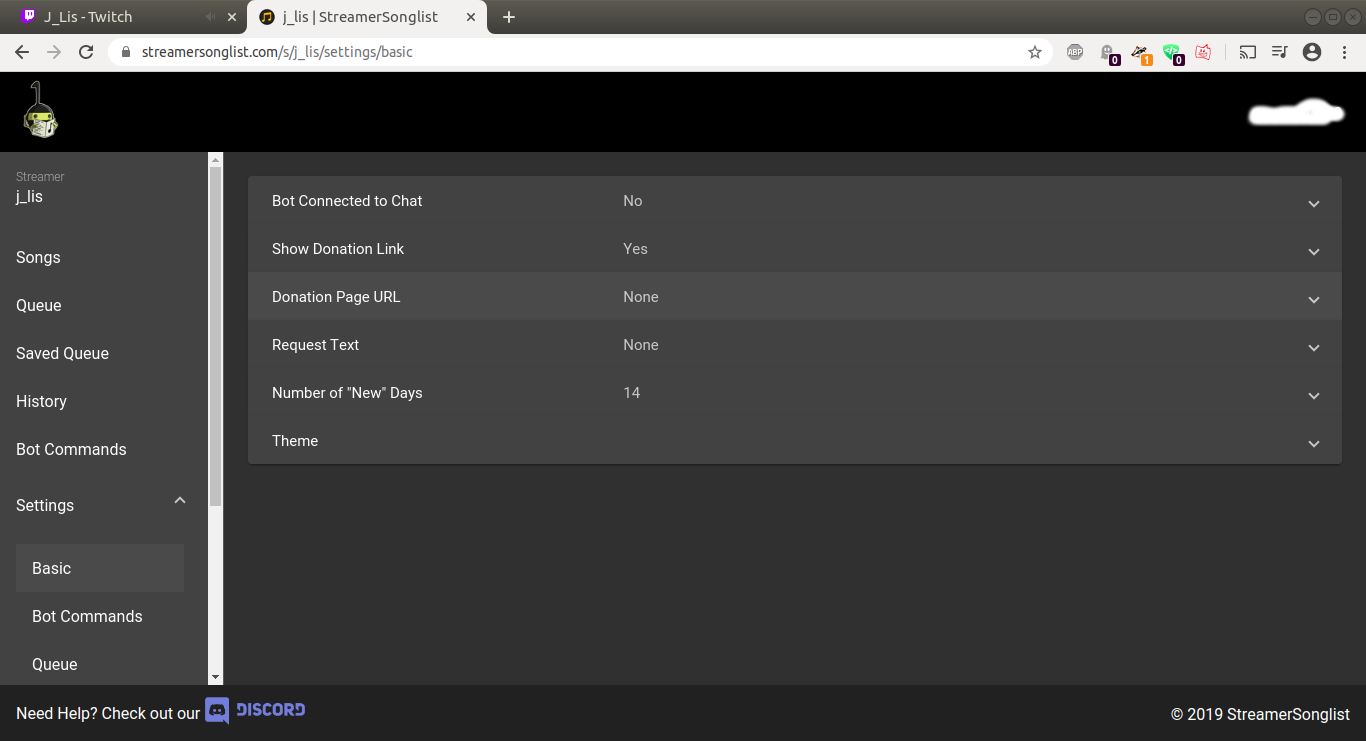
\includegraphics[width=\linewidth]{src/troubleshooting_songbot/bot_disconnected.png}
  \caption{The webpage with the songbot disconnected}
  \label{bot disconnected}
\end{figure}
When the bot is connected and it did not work, check the command list. songlist and songrequest have been known to get turned off by mods unknown.
\begin{figure}[ht!]
  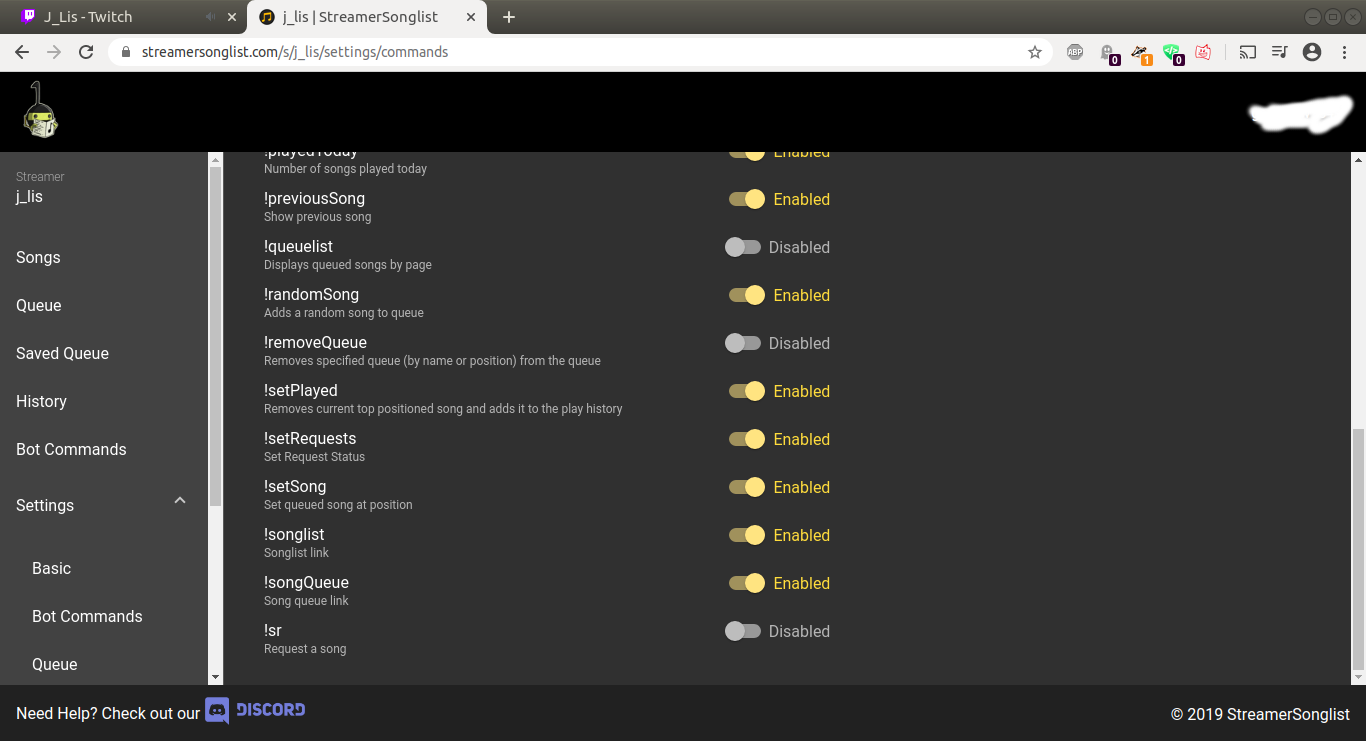
\includegraphics[width=\linewidth]{src/troubleshooting_songbot/songlist_commands_off.png}
  \caption{The webpage with the commands turned off}
  \label{commands off}
\end{figure}

\newpage
\subsection{What it is supposed to look like}
\begin{figure}[ht!]
  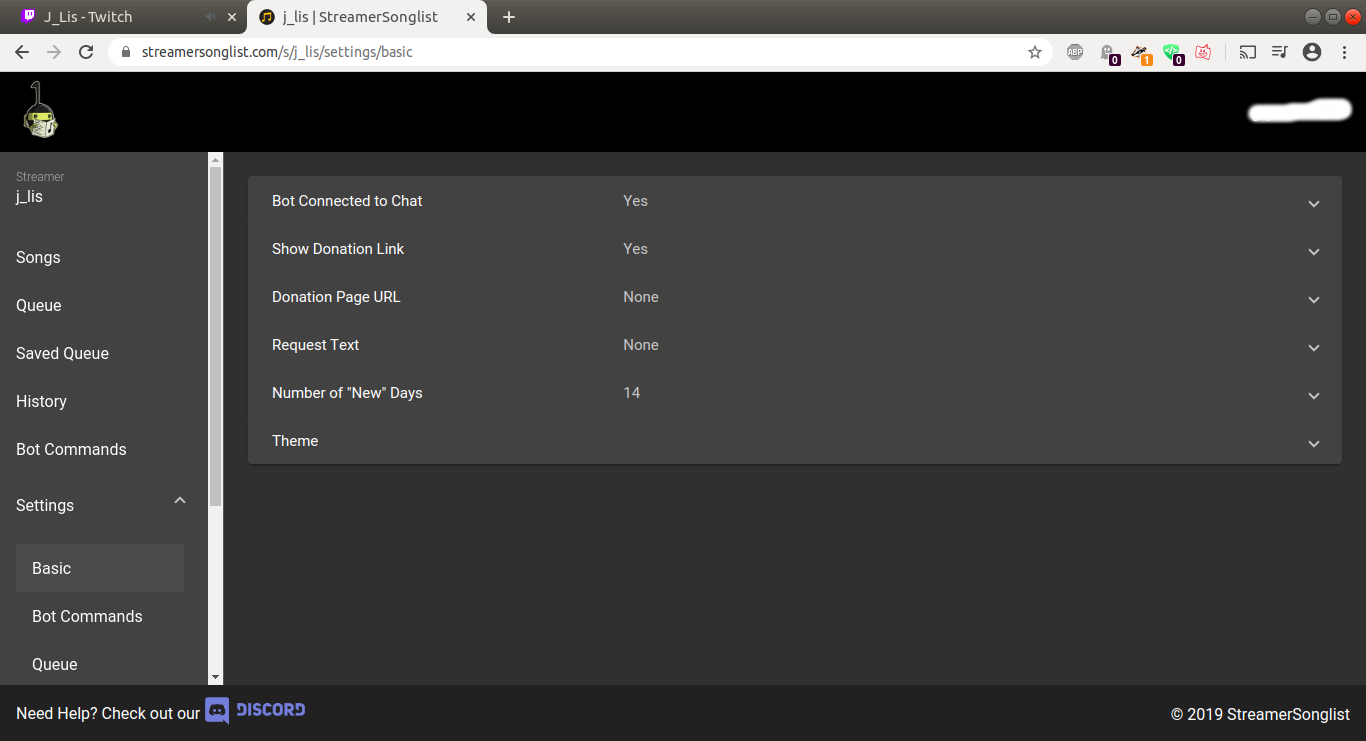
\includegraphics[width=\linewidth]{src/troubleshooting_songbot/bot_connected.png}
  \caption{The webpage with the songbot connected}
  \label{bot disconnected}
\end{figure}
\begin{figure}[ht!]
  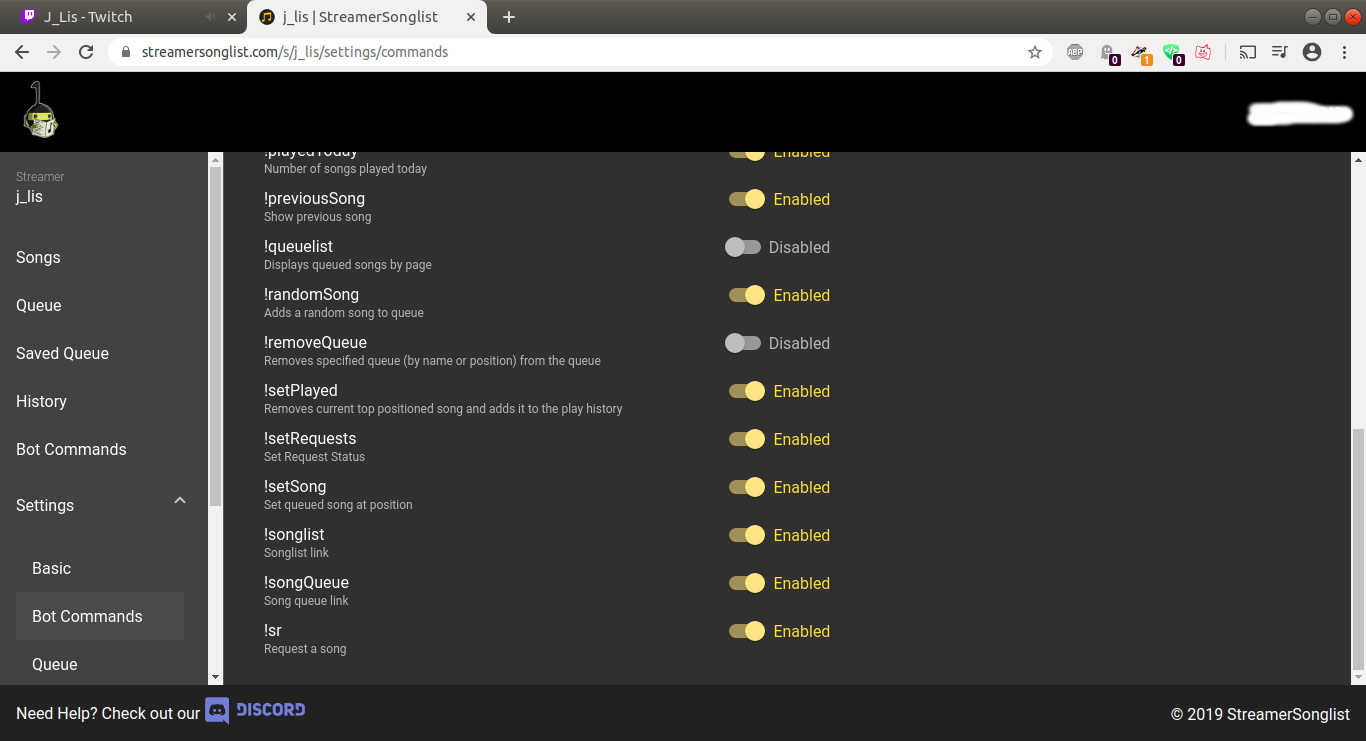
\includegraphics[width=\linewidth]{src/troubleshooting_songbot/songlist_commands_on.png}
  \caption{The webpage with the commands turned on}
  \label{commands off}
\end{figure}
\begin{figure}[ht!]
  \includegraphics[width=\linewidth]{src/troubleshooting_songbot/bot_on.png}
  \caption{The webpage with the songbot turned on}
  \label{bot is on}
\end{figure}




\end{document}
